\documentclass[11pt,twocolumn]{ieee}


% \input{new-commands}
\usepackage{latexsym}
\usepackage{times}
\usepackage{psfrag}
\usepackage{subfigure}
\usepackage{graphicx}
\usepackage{algorithm}
\usepackage{algorithmicx}
\usepackage{times}
\usepackage{epsfig}
\usepackage{graphicx}
\usepackage{amsmath}
\usepackage{amssymb}
\usepackage{mathtools}
\usepackage[utf8]{inputenc}
\usepackage[margin=1in]{geometry}
\usepackage[english]{babel}
\usepackage[breaklinks=true,bookmarks=false]{hyperref}


\newcommand{\RemarkRef}[1]{Remark~\ref{#1}}
\newcommand{\FigRef}[1]{Figure~\ref{#1}}
\newcommand{\AlgRef}[1]{Algorithm~\ref{#1}}
\newcommand{\TabRef}[1]{Table~\ref{#1}}
\newcommand{\UpStar}[1]{\overset{\ast}{#1}}
\newcommand{\CorRed}{\color{black}}
\newcommand{\EqRef}[1]{Eq.~(\ref{#1})}
\newcommand{\xly}[1]{\textcolor{red}{\textbf{XLY:} #1}}
\newcommand{\argmin}{\mathop{\rm argmin}}


\def\y{\mathbf{y}} %new added
\def\z{\mathbf{z}} %new added
\def\x{\mathbf{x}} %new added
\def\X{\mathbf{X}} %new added
\def\w{\mathbf{w}} %new added
\def\W{\mathbf{W}} %new added
\def\Wstar{\mathbf{W^{*}}} %new added
\def\p{\mathbf{p}} %new added
\def\pstar{\mathbf{p^{*}}} %new added
\def\P{\mathbf{P}} %new added
\def\Pstar{\mathbf{P^{*}}} %new added
\def\q{\mathbf{q}} %new added
\def\qstar{\mathbf{q^{*}}} %new added
\def\Q{\mathbf{Q}} %new added
\def\Qstar{\mathbf{Q^{*}}} %new added
\def\f{\mathbf{f}} %new added
\def\F{\mathbf{F}} %new added
\def\prob{\mathbb{P}} %new added
\def\D{\mathcal{D}} %new added
\def\S{\mathbf{S}} %new added
\def\mc{\mathcal} %new added
\def\nb{\boldsymbol{\nabla}} %new added


\DeclarePairedDelimiter\abs{\lvert}{\rvert}
\DeclarePairedDelimiter\norm{\lVert}{\rVert}

\newtheorem{theorem}{Theorem}
\newtheorem{thm}{Theorem}
\newtheorem{dfn}{Definition}
\newtheorem{lem}{Lemma}

%\textheight 9.1in

\title{Asynchronous Interactive Distributed Private Multitask Learning Framework with Trustworthy Data Aggregator}

\author{Liyang Xie\and Manni Liu\\
}

\begin{document}
\maketitle


\begin{abstract}
%!TEX root = main.tex

Recently, multi-task learning (MTL) has proved to be an powerful learning framework that improves performance in supervised learning problems by transferring knowledge among those tasks. Distributed MTL is one popular setting where the data is separated across different locations. The issue of privacy arises when distributed MTL is applied on geographically separated data. These data are usually personal data such as financial and medical records, which may contain personal sensitive information. In such case, privacy-preserving distributed MTL frameworks are in great need as the proliferation of private data. Differential privacy (DP) is one of the most important privacy concepts that are suitable for this type of framework. In this proposal, we put up with a novel idea: \textbf{A}synchronous \textbf{I}nteractive \textbf{D}istributed \textbf{P}rivate \textbf{M}ultitask \textbf{L}earning \textbf{F}ramework with Trustworthy Data Aggregator (AIDPMTLF) to address the privacy issue under distributed MTL setting. The proposed framework adds carefully designed perturbation on the data aggregator. We also provide theoretical guarantees of the proposed framework and extensive empirical results to illustrate our idea. 
\end{abstract}


\section{Introduction}
%!TEX root = main.tex

MTL has become a provalent tool in dealing with the problem of learning from the distributed data in the epoch of big data. In spite of its proliferation, challenges also arise. One indispensable challenge is about how the privacy of sensitive data is protected in distributed MTL framework. For example, medical centers in different countries may make a joint effort to conduct medical research, while the data may not be distributed because of its sensitive nature.

On sight, it seems that erasing personal information such as names can protect individual privacy. However, as the development of machine learning algorithms, it is still possible to extract patterns from remaining information and obtain personal information. Back to 2007, the famous media service provider Netflix published an anonymous dataset called Netflix Prize dataset, and encouraged researchers to design a better recommendation system. The dataset contains 10 million movie rankings from 500,000 customers. However, even customers' personal details like usernames and locations are removed and replaced by random numbers, some information is still deanonymized by comparing rankings and timestamps with public resources from the Internet Movie Database (IMDb)~\cite{4531148}. Other works also demonstrate it. \cite{doi:10.1111/j.1748-720X.1997.tb01885.x} and \cite{DBLP:journals/corr/abs-0803-0032} can extract hidden information from an adversary. Even genetic datasets can leak personal information\cite{10.1371/journal.pgen.1000167,Wang:2009:LYI:1653662.1653726}.

% \cite{Backstrom:2007:WAT:1242572.1242598} proves that a family under attack can be performed to social network nodes anonymized. 

As early as 1977, \cite{dalenius1977towards} has defined a concept for the ideal database: nothing about an individual that can not be learned without the database should be learned from the database. Although the idea is too demanding and is later demonstrated theoretically that this desideratum can not be reached\cite{Dwork06differentialprivacy}, effort can still be done to reduce the risk of leaking personal information stored in the dataset. In a word, differential privacy aims at maximizing the accuracy of queries to a database while minimizing the possibility of identifying a single record.

In this paper, we proposed a new method to address the issue arising from Smith {\it et al.}~\cite{smith2017interaction}. In~\cite{smith2017interaction}, the authors provided the answer to the question: "how much interaction is necessary to optimize convex functions in the local DP model?". Although this non-interactive setting achieves good performance, the testing result under the scenario of distributed MTL with trustworthy aggregator is far from satisfying. This is due to the fact that multitask learning aims at improving each user's performance with the help from all the others, which requires a lot of information exchange. Also in real world cases, heterogeneity of local data and tasks make it very hard to finish training in a few rounds. In addition, a method with few interactive or non-interactive typically requires a large amount of local datasets. This is hard to achieve due to the scarcity of the data under distributed MTL senses. 

In this paper, we will show that, with a trustworthy data aggregator, asynchronous interaction performs better than the proposed one in~\cite{smith2017interaction} . In addition, \cite{smith2017interaction} mentioned that it is difficult to implement an interactive framework for private data learning because of two reasons: (1) long network latency; (2) the server has to be online for asynchronous updates. The first issue can be addressed with the asynchronous update, whose effect will be further reduced with weighted update mechanism we proposed. The second issue can be addressed by data backup, which is easy to achieve because the complexity of the algorithm in aggregator is moderate.

In summary, this paper makes the following contributions:
\begin{itemize}
  \item We present the first distributed private learning system with fast light-weight interactions under the condition of a trustworthy central data processor.
  \item We carefully design the noise perturbation algorithm that is added on the aggregator and prove that the proposed algorithm guarantees local differential privacy (LDF)~\cite{duchi2013local}--one of the most important variants of DP. We check the correctness of our method using state-of-the-art tool~\cite{ding2018toward}.
  \item We reduce the accumulation effect of privacy leakage during iterative updates. We also explore the effect of different distributions of the delay and use weights to eliminate the effect of the delay as well as exploring other delay-reduce methods.
  \item We demonstrate our method with sufficient empirical evidences, which contain multiple real world settings such as task heterogeneity and data heterogeneity, 
\end{itemize}

The paper is arranged as follows: we first introduce the related work in section 2 with respect to differential privacy and distributed rrivate learning. Next in section 3, we give a detailed description on our model and method. Experiments results are provided in section 4, as well as analysis. We also discuss our technical Weaknesses and potential future work in section 5. We conclude our work in section 6 and provide details on project group members in section 7.
% The lower complexity than~\cite{smith2017interaction}
% The results are better than the non-interactive one presented in ~\cite{smith2017interaction}



\section{Related Work}
%!TEX root = main.tex

\textbf{Differential privacy.} Enormous algorithms have been proposed for privacy-preserving data mining\cite{Agrawal:2000:PDM:335191.335438,Evfimievski:2003:LPB:773153.773174,Sweeney:2002:KAM:774544.774552,Machanavajjhala:2007:LDP:1217299.1217302}. But composition attacks and auxiliary information become big problem for these algorithms. On the other hand, differential privacy acts as an resistance against composition attacks and auxiliary information.

When differential privacy is first put forward by C.Dwork\cite{Dwork:2006:CNS:2180286.2180305}, a sensitivity method is also introduced. If we denote the objective function as $J$ and the true query result coming from algorithm $\mathcal{A}$ is represented by $\mathcal{A}(D) = argmin\ J $, the output query result is $\mathcal{A}(D)+b$ where $b$ is an random noise with density $\frac{1}{\alpha} e^{-\beta \norm{b}}$. $\beta$ is a function of $\epsilon$ and the $L_2$-sensitivity of $\mathcal{A}(\cdot)$. The sensitivity method is a typical output perturbation method.

As for the objective perturbation methods, the objective function is turned to be $J(f,D)+\frac{1}{n}b^T f$ where $f$ is the predictor and $n$ is the number of training data points. If the objective function is strongly convex with some constraints on the loss function, objective perturbation proves theoretically better than output perturbation. More details can be found in \cite{Chaudhuri:2011:DPE:1953048.2021036}.

\textbf{Distributed Private Learning.} 
There are also important studies on distributed differentially private Learning. Xie {\it et al.}~\cite{xie2017privacy} for the first time, provide a privacy-preserving distributed MTL framework combined with distributed asynchronous MTL framework. The proposed method successfully address the issue of time delay caused by synchronized optimization algorithms. It is different from our settings because it assumes that the central server is untrustworthy and adding noise from local task side may significantly reduce the overall performance. Xie {\it et al.}~\cite{xie2016data} proposed a ensemble learning method for merging binary classifiers (or regressors) trained on local data. This method, though can be applied in our paper's setting with ''public-private" case, does not help much due to data heterogeneity. In~\cite{xie2016comparison} the authors proved that the method~\cite{xie2016data} has near-optimal performance under certian conditions. Han {\it et al.}~\cite{han2017differentially} present a distributed optimization algorithm (with constrained domain) that preserves differential privacy. This method may not achieve good performance due to its exponential mechanism. Rajkumar and Agarwal~\cite{rajkumar2012differentially} describe a new differentially private algorithm for the multiparty setting that uses a stochastic gradient descent based procedure to directly optimize the overall multiparty objective. This paper does not address the issue of accumulation effect of privacy leakage. Hamm {\it et al.}~\cite{hamm2016learning} proposed a method of building a global
differentially private classifier from locally classifiers from multiple local users without access to their private data. Similar as~\cite{xie2016data}, it does not help due to data heterogeneity. Pathak {\it et al.}~\cite{pathak2010multiparty} proposed a privacy-preserving framework for composing a differentially private aggregate
classifier using local trained classifiers by separate mutually untrusting
parties. This method requires other encryption method, which may lead to more cost.




\section{Methodology}
%!TEX root = main.tex

In this study we aim to provide solution to distributed MTL problems with asynchronous interaction between local learning models and a trustworthy central server. In the following sections we first describe the regularized MTL and analyze its distributed version, which is the foundation of our framework. Next we introduce the concept of DP and describe its importance in machine learning. Then we show that DP is an indispensable part of the proposed framework. With necessary precondition and assumptions, we provide detailed description of our framework.

\subsection{Regularized MTL and Its Distributed Version}

The relatedness among learning tasks is the foundation of MTL. In our settings we assume that there are totally $T$ tasks. Let $d$ be data dimension and $n_{t}$ be the number of data points in task $t$, task $t$ contains a dataset $\mathcal D_{t} = \{X_{t},\y_{t}\}$, where $X_{t} \in \mathbb R^{n_{t}\times d}$ is the data
matrix with feature dimensionality $d$, $\y_{t} \in \mathbb R^{n_{t}}$ is the
corresponding label vector. For each local task, a model
$f(\x; \w): \mathbb R^{d} \rightarrow \mathbb R$ is learned. To predicts $y$, we use learned $\w$ and feature vector $\x$ in testing set. Note that we use linear model in this paper and hence $f(\x; \w) = \x^T\w$. Let
$\ell_{t,i}(\w_{t}) = \ell(f(\x_{t,i}; \w_{t}), y_{t,i})$ be the loss
for the task $t$'s $i$th sample with loss function $\ell$. Let $W = [\w_1, \dots, \w_T] \in \mathbb
R^{d \times T}$ be the model matrix whose $i$th column is the task model
$\w_{t}$. Regularized MTL solves the following problem:
% \begin{align} 
% \min_{W} \left\{ \sum\nolimits_{t=1}^T \left(\frac{1}{n_{t}}\sum\nolimits_{i=1}^{n_{t}} \ell_{t,i}(\w_{t})\right) + \lambda r(W) \right\}
% \label{eqt:mtl}
% \end{align}
\begin{align} 
\min_{W} \left\{ \displaystyle{\sum_{t=1}^T} \left(\frac{1}{n_{t}}\displaystyle{\sum_{i=1}^{n_{t}}} \ell_{t,i}(\w_{t})\right) + \lambda r(W) \right\}
\label{eqt:mtl}
\end{align}
Here $r(\W)$ serves as the regularization to induce task relatedness according to different relatedness assumptions~\cite{argyriou2008convex, kim2010tree}. $\lambda$ is the parameter that determines the strength of knowledge transfer. This is centralized version of MTL.

An alternative representation of~\ref{eqt:mtl} is the following:
% \begin{align}
% \min_{P, Q} \left\{ \sum\nolimits_{t=1}^T \left(\frac{1}{n_{t}}\sum\nolimits_{i=1}^{n_{t}}
% \ell_{t,i}(\p_{t} + \q_{t})\right) + \lambda r(P) + \tau g(Q), \right\}\label{eqt:mtl_pq}
% \end{align}
\begin{small}
\begin{align}
\min_{P, Q} \left\{ \displaystyle{\sum_{t=1}^T} \left(\frac{1}{n_{t}} \displaystyle{\sum_{i=1}^{n_{t}}}
\ell_{t,i}(\p_{t} + \q_{t})\right) + \lambda r(P) + \tau g(Q) \right\}\label{eqt:mtl_pq}
\end{align}
\end{small}
where $\w_{t} = \p_{t} + \q_{t}$ and $W = P + Q$. $r(P)$ performs the knowledge transfer and $g(Q)$ regulates the model complexity. The motivation of this representation is that in MTL setting, the knowledge of learned parameter $\w_{t}$ contains two components: a shared component $\p_{t}$ that comes from tasks other than $t$ and a task specific component $\q_{t}$ that contains the local knowledge. This approach provides the flexibility to trade off between the shared one and the task specific one during training. 

Our goal now is to make~\ref{eqt:mtl_pq} into a distributed version such that it can be solved with distributed learning techniques. Following is the proximal operator that can help transforming \ref{eqt:mtl_pq} into a distributed fashion:
\begin{align}
\text{prox}_{r}^{\mu}(X) = 
     \argmin\nolimits_{W} \left\{\tfrac{1}{2}\|W-X\|_{F}^{2} + \mu r(W) \right\},
\label{def:prox}
\end{align}
where $\mu$ is a coefficient obtained by the step size and the regularization parameters, and $r(W)$ is required to be a proper and lower semi-continuous function.

With definition~\ref{def:prox}, representation \ref{eqt:mtl_pq} can be expressed as the following distributed version:
\begin{align}
Q^+ &= Q^- - \alpha \nabla_Q f(Z^-)
    \label{eq:mtl_prox_q}\\
P^+ &= \text{prox}_{r}^{\alpha\lambda}(P^- - \alpha \nabla_P f(Z^-))
    \label{eq:mtl_prox_p}
\end{align}
where $f(Z)$ is the loss function which has the following expression:
% \begin{align*}
% \begin{split}
% f(Z) &= f(P, Q)\\
% &= \sum_{t=1}^T \left(\frac{1}{n_{t}}\sum\nolimits_{i=1}^{n_{t}}
%  \ell_{t,i}(\p_{t} + \q_{t})\right) + \tau g(Q).
% \end{split}
% \end{align*}
\begin{align*}
\begin{split}
f(Z) &= f(P, Q)\\
&= \sum_{t=1}^T \left(\frac{1}{n_{t}}\displaystyle{\sum_{i=1}^{n_{t}}}
 \ell_{t,i}(\p_{t} + \q_{t})\right) + \tau g(Q)
\end{split}
\end{align*}
where $Z = \begin{bmatrix}
P \\ Q 
\end{bmatrix}  \in \mathbb R^{2d \times T}$
is the parameter vector.

The above steps are indeed easy to be distributed: $Q$ can be decoupled and distributed for each task for fixed $p_t$. The $t$th local task receives the current shared component $\p_t^-$ from the central server, computes
the gradient $\nabla_{\p_t} f(Z^-)$ (using task data $\mathcal D_t$), sends it back 
to the server, and finally locally updates $\q_t^+$ using its data. We note that 
the gradient $\nabla_{\p_t} f(Z^-)$ can be computed locally because of the following:
% \begin{align*}
% \begin{split}
% \nabla_{\p_t}f(Z) &= \nabla_{\p_t}f(\p_t, \q_t) \\
% &= 
% \nabla_{\p_t} \left\{ \frac{1}{n_{t}}\sum\nolimits_{i=1}^{n_{t}}
%  \ell_{t,i}(\p_{t} + \q_{t}) + \tau g_i(\q_t) \right\}
% \end{split}
% \end{align*}
\begin{align*}
\begin{split}
\nabla_{\p_t}f(Z) &= \nabla_{\p_t}f(\p_t, \q_t) \\
&= 
\nabla_{\p_t} \left\{ \frac{1}{n_{t}}\displaystyle{\sum_{i=1}^{n_{t}}}
 \ell_{t,i}(\p_{t} + \q_{t}) + \tau g_i(\q_t) \right\}
\end{split}
\end{align*}
where the computation only depends on the task data $\mathcal D_t$. After all the gradients $[\nabla_{\p_1} f(Z^-), \dots,
\nabla_{\p_T} f(Z^-)]$ are received, the server immediately performs proximal computation
as in Equation~\eqref{eq:mtl_prox_p}, and then sends the columns to the corresponding
task nodes. 

\subsection{The Necessity of Privacy and Differential Privacy}
\label{Necessity}

Data such as financial records and patients' MRI images contain sensitive information, which raises privacy issues in machine learning. Therefore it is necessary to take the issue of data privacy into consideration. The \textit{fundamental assumptions} in our framework are: (1) data aggregator is trustworthy, (2) communication channels are trustworthy, (3) local tasks are not trustworthy, which is very different from the settings in Xie {\it et al.}~\cite{xie2017privacy}. Our setting widely appears in real world scenario and hence solving it will make great contribution. In our framework, the gradient $\nabla_{\p_t}f(\p_t^-, \q_t^+)$ sent to the data aggregator contains private information from local task. However there is not need to add noise before sending out the gradient due to the trustworthy aggregator. After the knowledge transfer in aggregator, the gradient send back to certain local task contains sensitive information from all the other local task, which requires privacy protection. 

In this paper, we aim to protect the \textit{differential privacy} of
each data point in each local task (formally defined in
Definition~\ref{thm:dp}). Differential privacy~\cite{dwork2006differential}
provides a quantifiable level of privacy with respect to the individual data
points. First we provide a mathematical definition of $\epsilon$-differential privacy which is very essential to differential privacy:

\begin{theorem}
\textbf{($\epsilon$-differential privacy\cite{Dwork:2014:AFD:2693052.2693053})}\indent Let $\epsilon$  be a positive real number and $\mathcal{A}$ be an randomized algorithm that takes a dataset $D$ as input. Let $\displaystyle {\textrm {im}}{\mathcal{A}(D)}$ denote the output of feeding D to $\mathcal{A}$ . The algorithm $\mathcal {A}$ is \textbf{$\epsilon$-differentially private} if for any two datasets $D_{1}$ and $D_{2}$ that differ on a single element (i.e., the data of one person), and all subsets $S$ of $\displaystyle {\textrm {im}}{\mathcal {A}}$,
\[Pr[\mathcal{A}(D_1)\in S]\leq \epsilon \times Pr[\mathcal{A}(D_2)\in S]]\]
where the probability is taken over the randomness used by the algorithm.
\label{thm:dp}
\end{theorem}

$\epsilon$-differential privacy is a privacy measurement which is famous for its robustness to know attacks and has been widely applied in subsequent research. In an intuitive way, an algorithm is regarded as satisfying $\epsilon$-differential privacy if modifying the data of one person doesn't effect the output distribution a lot. Since most differential privacy algorithms are designed on the basis of adding noises to the original dataset, the degree of how much privacy is violated can be quantified with this theoretical definition, and thus we can measure the effectiveness of an algorithm. 

% In general, there are two directions for designing $\epsilon$-differential privacy algorithms: output perturbation\cite{Dwork:2006:CNS:2180286.2180305} and objective perturbation\cite{Chaudhuri:2011:DPE:1953048.2021036}. When a true result is obtained from a query to a database, output perturbation protects privacy by adding noises to the true result and then returns the true result plus noises to users. On the other hand, objective perturbation adds noises to the regularized empirical risk minimization objective function before optimizing it.

\subsection{Differentially Private Distributed MTL}

As we mentioned in section~\ref{Necessity}, privacy issue in the non DP framework requires us to propose a privacy-preserving framework such that it can not only transfer accurate information among learning task to help improve performance but also provide privacy guarantee. Our idea is to add noise on the matrix ($P^+$ in~\ref{eq:mtl_prox_p}) such that the returned gradients are perturbated. The perturbation method is under developed. We summarize our idea in Figure~\ref{fig:framework}.
\begin{figure}
\centering
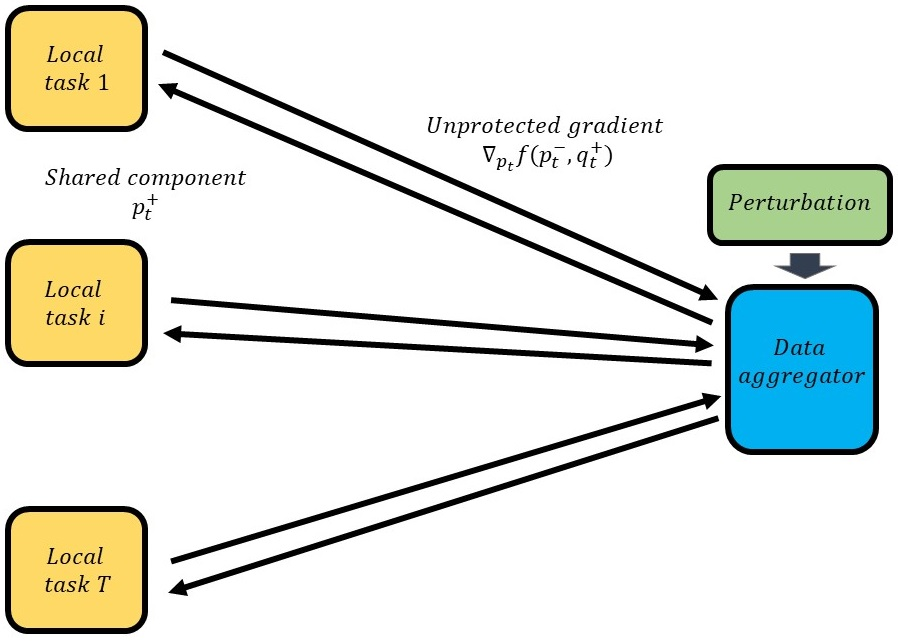
\includegraphics[scale=0.35]{figure/framework.jpg}
\caption{Proposed framework.}
\label{fig:framework} 
\end{figure}



\section{Experiments and Discussions}
%!TEX root = main.tex
% Data set should be small here due to our settings.

We first present the convergence of proposed method and baseline under non-private and private cases, under synthetic data on the centrallized MTL framework.

We then present the convergence of proposed method and baseline under non-private and private cases, under synthetic and real data.

Privacy and delay


\section{Future work}
%!TEX root = main.tex

\textbf{AIDPMTLF} can learn big data well while protecting the private information as shown in section 4. However, the protection of privacy never stops as attack models arises and develops everday. For the future work, we still consider differential privacy as perspective for multi-task learning problems. Further contribution can be made from: 1) specfic model design for specific datasets. Because each dataset faces different attacks. For example, Netflix Prize dataset is threatened as the existence of public resources from the Internet Movie Database. Financial and medical records all face different information leakage ways. \textbf{AIDPMTLF} disolve the privacy issue in a general case. More specific modication can be made on the basis of it when facing different multi-task learning problems. 2) Noises can be analyzed and used to improve the model. Feedback mechanism may produce promotion. 3) Different network structures may incur unexpected results. We use basic neural networks in this paper. Creative network design is promising for amazing achievement for big data analysis.


\section{Conclusion}
%!TEX root = main.tex

In this paper, we highlight the contribution of  multi-task learning on current research of big data analysis. But we also analyze the limitations of it on private datasets. Privacy has been an enduring topic in computer science and appeals a lot of concentration. We introduce differential privacy and emphasize its good performance on privacy-preserving. By combing multi-task learning and differential privacy, we come up with a model called Asynchronous Interactive Distributed Private Multitask Learning Framework with Trustworthy Data Aggregator (AIDPMTLF). Experiments in section 4 reveals its good performance on big data while protecting the data privacy. We further analyze its weakness and discuss the future work.


\section{Appendix}
%!TEX root = main.tex

Liyang Xie: Methodology part, experiment part, paper revision. 

Manni Liu: Background Survey, presentation part, paper revision. 


\bibliographystyle{IEEE}
\bibliography{ieee}


\end{document}
